\chapter{Background}
\label{cha:background}

% Software vs. Security
% Risk and vulnerability and CVEs
% Industrial Control Systems (ICS) and Operational Technology (OT)
% Industrial Internet of Things (IIoT)
% Difference Between IT and OT Security
% Devices and Constraints
% What Is a Security Scan

This chapter contains an explanation of many fundamentals terms used in the thesis, without which it would not be possible to fully understand all the covered topics. 

\section{Software vs. Security}

A software is a set of programs and data which provides functionalities. Security is understanding and identifying software-induced security risks and how to manage them. Software and functionalities come with certain risks and the software security is about managing these ones.

Therefore, software plays a crucial role in providing security, but it is also one of the relevant source of security issues and problems. Many times the developers have a limited training on this concept or many times the goal is the speed of the development rather than the attention to the \textit{hidden} details; as result, security is always considered a secondary factor, because it is a complex and expansive task, hard to evaluate when nothing bad happens but usually too late to evaluate when something bad happens.~\cite{st-slides}

A software system is secure if it satisfies specified security objectives, starting from the CIA triad:
\begin{itemize}
  \item \textbf{Confidenziality}: unauthorized actors cannot have access or read the information;
  \item \textbf{Integrity}: unauthorized actors cannot change or alter the information;
  \item \textbf{Availability}: authorized actors can always have access to the information;
\end{itemize}
The CIA triad is a common model that forms the basis for the development of security systems. It is used for finding vulnerabilities and methods for creating solutions. This differentiation is helpful because it helps guide security teams as they pinpoint the different ways in which they can address each concern.\\
Ideally, when all three standards have been met, the security profile of the organization is stronger and better equipped to handle threat incidents.~\cite{cia-triad}

A secure software is not only composed of the CIA triad; there are also other objectives like~\cite{st-slides}
\begin{itemize}
  \item \textbf{Authentication}: who is performing a task;
  \item \textbf{Authorization}: what is that actor allowed to do;
  \item \textbf{Privacy}: controlling personal information from being shared;
  \item \textbf{Anonymity}: remaining unidentified to others;
  \item \textbf{Non-repudiation}: actor cannot deny having taken an action;
  \item \textbf{Reliability}: the extent to which a software yields consistent and results as expected;
  \item \textbf{Audit}: having traces of performed actions in separate systems or places;
  \item \textbf{Monitoring}: observing the system for any unusual activity;
  \item \textbf{Intrusion detection}: detecting unauthorized access;
  \item \textbf{Intrusion prevention}: stopping unauthorized access;
  \item ...and so on
\end{itemize}

Total security is unachievable, but the goal is to minimize the risks and the vulnerabilities. The security is a process, not a product, and it is a continuous process.~\cite{st-slides}

\section{Risk vs. vulnerability vs. CVE}

We talked about risks in the previous section, but what is a risk? A risk is the potential that a dangerous situation becomes reality. It is the probability of a threat exploiting a vulnerability and the impact of that event. A risk is a combination of a threat, a vulnerability, and an impact.

Safety is about protecting from accidental risks, while security is about mitigating the risk of dangers caused by intentional and malicious actors.

A system is secure as its weakest element. A vulnerability is a weakness in a system that can be exploited by a threat. A threat is a potential danger that can exploit a vulnerability. A threat agent is the actor that can exploit a vulnerability. An attack is the exploitation of a vulnerability by a threat agent. An exploit is the code that takes advantage of a vulnerability.

CVE, which stands for \textit{Common Vulnerabilities and Exposures}, is a list of publicly known cybersecurity vulnerabilities. The CVE system provides a reference-method for publicly known information-security vulnerabilities and exposures. Each CVE entry represents a unique identifier for a specific vulnerability, named \textit{CVE-ID}, making it easier to reference it accross different tools. 

An entry is rated via the CVSS score, namely the Common Vulnerability Scoring System, which is a method used to supply a qualitative measure of severity. CVSS is not a measure of risk. CVSS v2.0 and CVSS v3.x consist of three metric groups: Base, Temporal, and Environmental. CVSS v4.0, released in 2023, is a bit different and consists of Base, Threat, Environmental and Supplemental metric groups. Metrics result in a numerical score ranging from 0 to 10. A CVSS assessment is also represented as a vector string, a compressed textual representation of the values used to derive the score.~\cite{cvss-metrics}

% TODO: Add CVEs for year or some statistics in general

NVD is the \textit{National Vulnerability Database}, a U.S. government database that contains information about known vulnerabilities, including their CVE identifiers and CVSS scores. It is maintained by NIST and serves as a comprehensive resource for organizations to evaluate security risks.

NIST (\textit{National Institute of Standards and Technology}) is a U.S. federal agency that develops cybersecurity standards, guidelines, and best practices. Even if it is an american agency, its standards are widely used around the world.

\subsection{Bugs}

A bug is a flaw in a system that is not behaving as it is designed to do.\\
A vulnerability is a way of abusing the system, in a security-related way, whether that's due to a design fault or an implementation fault, so a bug.

Many security issues are related to vulnerabilities due to bugs, but not all bugs are vulnerabilities. The exploitation is the activity composed by many steps in which an attacker uses a bug to gain its goal.

\section{IT and OT Security}
 
IT (\textit{Information Technology}) and OT (\textit{Operational Technology}) focus on protecting different types of systems and they have distinct priorities. 

IT focuses on managing electronic data, while OT is centered on controlling physical processes and equipment. To better explain, IT is essential for business operations and decision-making and involves the use of computers and software to gather, store, process, share data securely. OT employs hardware and software to monitor and control industrial operations, ensuring efficiency and safety in sectors like manufacturing and energy. It is distinct from Information Technology (IT) as it directly interfaces with industrial equipment and processes, focusing on the physical environment and operational needs.~\cite{paloalto-it-ot-diff}

We can devise some comparison points between the two types:

\subsection{Primary priorities}

IT security prioritizes Confidentiality, Integrity and Availability (CIA), with the main focus set to protect data from breaches and authorized actions, while OT security prioritizes Availability, Integrity and Confidentiality (AIC), ensuring the continuous operation of critical systems with safety and reliability being more important than data confidentiality.

\subsection{Impact of Security Breaches}

IT breaches tipically affect data confidentiality and may result in privacy violations, financial losses or business disruptions. OT breaches can have severe direct consequences, including physical damage and environmental harm.

\subsection{Security Measures}

IT security can use cybersecurity tools such as firewalls, antivirus, encryption and user authentication. Instead, OT security should require specialized tools like network segmentation, strict access control and real-time monitoring.

\subsection{Regulatory Requirements}

The former uses regulations like GDPR, the \textit{General Data Protection Regulation} to protect personal data for an European citizen and standards like ISO-27001, while the latter follows regulations and standards like the IEC 62443, which is a series of standards for industrial automation and control systems management and security. More on these regulations in the next chapters.

\subsection{Vulnerability management}

IT systems can usually be patched with a software update in a short time without severe impact on operations, while OT systems may require a longer time to be patched, as they are often critical to the operation of industrial processes or incompatible with the running legacy systems.


Despite their distinct differences, IT vs. OT cybersecurity share similarities and are increasingly overlapping and one approach have not to exclude the other.

According to the \textit{2023 State of Operational Technology and Cybersecurity Report} by Fortinet\footnote{\url{https://www.fortinet.com/}}, as shown in~\cref{fig:fortinet-intrusions-env-impacted}, nearly one-third of of respondents indicated both IT and OT systems were impacted, up from the 21\% in 2022.

\begin{figure}[h]
  \centering
  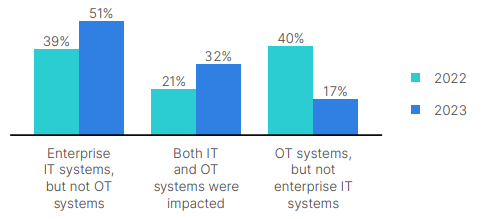
\includegraphics[scale=0.8]{chapters/02/assets/fortinet-intrusions-env-impacted.png}
  \caption[Environments impacted]{Environments impacted}
  \label{fig:fortinet-intrusions-env-impacted}
\end{figure}


As a general rule, OT devices are traditionally kept separate from the public internet and often internal networks, which meant they could only be accessed by authorized employees. However, it is increasingly possible for OT systems to be controlled and monitored by IT systems or remotely via the internet.~\cite{it-vs-ot-cybersecurity}

\section{Industry 4.0}

Industry 4.0, synonymous of \textit{smart manufacturing}, is the realization of the digital transformation of the field, delivering real-time decision making, enhanced productivity, flexibility and agility to revolutionize the way companies manufacture, improve and distribute their products.  

This is the Fourh Industrial Revolution, characterized by increasing automation and the employment of smart machines and smart factories. By collecting more data from the factory floor and combining that with other enterprise operational data, a smart factory can achieve information transparency and better decisions.

Some specific technologies are pushing this revolution:~\cite{what-is-industry-4-0}
\begin{itemize}
  \item \textbf{Internet of Things (IoT)}: machines on the factory floor are equipped with boars that allows the machines to connect with remote services, making possible to large amounts of valuable data to be collected, analyzed and exchanged.
  \item \textbf{Cloud computing}: the typically large amount of data being stored and analyzed can be processed efficiently and cost-effectively with cloud. Cloud computing can also reduce startup costs for small- and medium-sized manufacturers who can right-size their needs and scale as their business grows.
  \item \textbf{AI and machine learning}: Artifical Intelligence (AI) and machine learning can create insights providing visibility, predictability and automation of operations and business processes. The data collected from these assets can help businesses perform predictive maintenance based on machine learning algorithms, resulting in more uptime and higher efficiency.
  \item \textbf{Edge computing}: to reduce latency and improve security, edge computing can be used to process the needed data closer to the source, rather than sending it all the raw statistics to the cloud, wasting bandwidth and time.
  \item \textbf{Cybersecurity}: last but not least, when undergoing a digital transformation to Industry 4.0, it is essential to consider a cybersecurity approach that encompasses IT and OT equipment.
\end{itemize}

\section{Devices: PLC and HMI}

Industrial devices are used in many different sectors like manufacturing, energy, transportation, and so on. We can trace back these devices to a common tablet placed on a wall or on a production line, with the difference that these devices support a wide range of industrial protocols. These devices are usually not connected to the internet and they take input from a physical human interaction directly on the place. 

This type of devices is called HMI, which stands for \textit{Human Machine Interface}, and they are defined as a feature or component of a certain device or software application that enables humans to engage and interact with machines.\\
Traditionally, in order to integrate a manufacturing line with an HMI, the HMI had to be connected to a Programming Logic Controller (PLC) and the HMI displayed the data received from the PLC and gave the PLC input from users.~\cite{what-is-hmi}

In terms of the demands of Industry 4.0, industrial HMIs will also see further incorporation of new and emerging technologies that are impacting HMIs as a whole. First of all, there is the need to start integrating the Internet of Things (IoT) into industrial HMIs. This will allow for the collection of data from the factory floor and the ability to analyze that data in real-time. This will also allow for the ability to control the factory floor from a remote location. Of course, making these devices connected to the internet makes the risks of cyberattacks higher.

\section{Security Scan}

A security scan is a process that looks for vulnerabilities in a system or network. It is a way to identify potential security risks and weaknesses that could be exploited by attackers. Security scans can be performed manually or automatically using specialized tools. The goal of a security scan is to identify vulnerabilities and provide recommendations for improving the security of the system.

There are different types of security scans, including network scans, vulnerability scans, and penetration tests. Network scans are used to identify devices on a network and detect open ports and services. Vulnerability scans are used to identify security vulnerabilities in software and systems. Penetration tests are used to simulate cyberattacks and test the security of a system.

Security scans are an important part of a comprehensive security program. They can help organizations identify and address security vulnerabilities before they are exploited by attackers. By regularly performing security scans, organizations can improve their security attitude and reduce the risk of a security breach.

\section{ICS and IACS}

ICS and IACS refer respectively to \textit{Industrial Control System} and \textit{Industrial Automation and Control Systems}. In our context, they can be used interchangeably to define the collection of hardware, software and policies that controls and manages the industrial process. Basically, it means that anything interacting with the system influencing its safety, security and operations belong to IACS.~\cite{ics-or-iacs}
